\chapter{Pr\'{e}sentation de l'entreprise}
\section{SAP dans le monde}

SAP, qui signifie \textquote{Systeme, Anwendungen und Produkte in der DatenverarbeitungSystems} ou \textquote{Systems Application and Products in data processing}, à été formé en 1972 par cinq anciens employés d'IBM et ont inventé l'ERP\footnote{Entreprise Ressource Planning} ou PGI en Français\footnote{Progiciel de gestion intégré}. Son siège est à Walldorf, en Allemagne. SAP conçoit et vend des logiciels de gestion et de reporting à destination des entreprises et des professionnels.\\

SAP est le premier éditeur de logiciels en Europe (devant Dassault Systèmes, Sage et Software AG)\footnote{Source : \url{http://www.journaldunet.com/solutions/dsi/truffle-100-europe-2014.shtml}} et le quatrième mondial (derrière Microsoft, IBM et Oracle)\footnote{Source : \url{http://www.journaldunet.com/solutions/ssii/classement-mondial-editeur-2010/editeur-logiciel-classement-mondial.shtml}}. Ses principaux concurrents sont les autres éditeurs d'ERP et de logiciels de gestion. Le chiffre d'affaire de l'année fiscale 2014 est de 17,56 milliards \texteuro.\\

SAP fournit plus de 293 000 clients venant de 190 pays et regroupe plus de 74 400 employés dans plus de 130 pays\footnote{Source : \url{http://www.sap.com/corporate-en/about/our-company/index.html}}. Pour plus d'informations à ce sujet consulter l'annexe \ref{annexe:SAP-Corporate-Fact-Sheet} page \pageref{annexe:SAP-Corporate-Fact-Sheet}\footnote{\url{http://www.sap.com/bin/sapcom/en_us/downloadasset.2015-07-jul-22-01.SAP-Corporate-Fact-Sheet-en-2015-07-22-pdf.html}}.\\
Les membres du conseil d'administration de SAP sont représentés dans le tableau page \pageref{table:board}.\\



\begin{table}[h!]
\small
	\begin{center}
     \begin{tabular}{ c  p{10cm} }
			 \raisebox{-\totalheight}{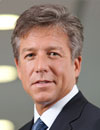
\includegraphics[height=0.1\textheight]{images/sap-executive-mcdermott.jpg}}
				& 
				\begin{itemize}
				\item Bill McDermott
				\item CEO
				\item a rejoint SAP en 2002
				\item a rejoint le conseil d'administration en 2008
				\item le terme de son mandat au conseil expire en 2017
				\item autres sièges en conseil d'administration : ANSYS, Inc ; Under Armour, Inc
				\end{itemize}
				\\ 
				
				\raisebox{-\totalheight}{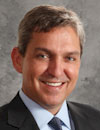
\includegraphics[height=0.1\textheight]{images/rob-enslin.png}}
				& 
				\begin{itemize}
				\item Robert Enslin
				\item Président, opérations client
				\item a rejoint SAP en 1992
				\item a rejoint le conseil d'administration en 2014
				\item le terme de son mandat au conseil expire en 2017
				\item responsabilités particulières : stratégie de marché, cloud, ventes régionales, ventes de l'industrie spécialisée, écosystème, expérience client end-to-end
				\end{itemize}
				\\ 
				
				\raisebox{-\totalheight}{
\includegraphics[height=0.1\textheight]{images/bernd-leukert.png}}
				& 
				\begin{itemize}
				\item Bernd Leukert
				\item produits et innovation
				\item a rejoint SAP en 1994
				\item a rejoint le conseil d'administration en 2014
				\item le terme de son mandat au conseil expire en 2017
				\item responsabilités particulières : organisation du développement global, analyse, application, cloud, bases de données et technologies, mobile
				\end{itemize}
				\\ 
				
				\raisebox{-\totalheight}{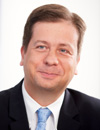
\includegraphics[height=0.1\textheight]{images/lika-mucic.png}}
				& 
				\begin{itemize}
				\item Lika Mucic
				\item Directeur financier, Directeur des opérations
				\item a rejoint SAP en 1996
				\item a rejoint le conseil d'administration en 2014
				\item le terme de son mandat au conseil expire en 2017
				\item responsabilités particulières : finance et administration, relations investisseurs et protection des données
				\end{itemize}
				\\ 
				
				\raisebox{-\totalheight}{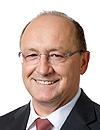
\includegraphics[height=0.1\textheight]{images/oswald.jpg}}
				& 
				\begin{itemize}
				\item Gerhard Oswald
				\item a rejoint SAP en 1981
				\item a rejoint le conseil d'administration en 1996
				\item le terme de son mandat au conseil expire en 2016
				\end{itemize}
				\\ 
				\end{tabular}
		\label{table:board}
	\end{center}
\end{table}
			
\clearpage
			
			

SAP mène une stratégie d'acquisition\footnote{Source : \url{http://www.sap.com/corporate-en/about/investors/newsandreports/acquisitions/index.html}} des leaders des technologies de l'information. La croissance organique étant le moteur de cette stratégie, tout en continuant à investir dans le développement de ses propres produits et dans les technologies innovatrices. Cette stratégie permet à SAP de mieux soutenir l'innovation en la dirigeant vers les partenaires possédant les domaines d'expertise requis. SAP perdure dans ce sens pour acquérir les technologies stratégiques cibles pour couvrir un marché toujours plus grand et pour satisfaire toujours plus les besoins de ses clients.
Le nouveau marché que vise SAP est celui du Big data, dans lequel nous pouvons l'imaginer leader dans quelques années.\\

La structure actuelle est le fruit du rachat de Business Objects par SAP France dont la date l\'{e}gale est le 1er janvier 2010, l'annonce ayant été faite le 7 octobre 2007. Pr\'{e}c\'{e}demment, Business Objects ayant absorb\'{e} deux autres entit\'{e}s, CARTESIS et Crystal decisions. Les rachats de SAP se succèdent : Sybase en 2010, SuccessFactors en 2011, Ariba et Syclo en 2012, Hybris en 2013, FieldGlass et pour finir Concur en 2014.\\







\subsection{Les produits SAP}
Les solutions logicielles de SAP\footnote{Source : \url{http://www.sap.com/france/pc/index.html}} sont principalement à destination des professionnels et offrent un grand nombre de logiciels destiné au traitement de tout type de problématique.\\
Historiquement, SAP est le leader (et inventeur) des progiciels, logiciels de gestion d'entreprise qui ont su, avec le temps, devenir incontournable pour toute moyenne ou grande entreprise.\\
En terme de logiciel de gestion, SAP propose :
\begin{itemize}
	\item Business suite
	\item Développement durable
	\item Gestion comptable et financière
	\item Progiciel de gestion intégré (ERP)
	\item Gestion de la chaine logistique (SCM)
	\item Gestion de la relation client (CRM)
	\item Gestion du cycle de vie des produits (PLM)
	\item Gestion des achats
	\item Gestion des actifs d'entreprise
	\item Gestion des ressources humaines (GRH)
\end{itemize}

Outre le fait de pouvoir organiser les flux d'information de l'entreprise, SAP s'est imposé comme l'un des leaders de l'analyse de ces données.\\
Parmi ces outils d'analyse, nous avons :
\begin{itemize}
	\item Analyse prédictive
	\item Applications analytiques
	\item Business intelligence
	\item Entrepôt de données (Data warehousing)
	\item Gouvernance, risques et conformité
	\item Pilotage de la performance
\end{itemize}

SAP se voulant une entreprise aux solutions complètes et innovantes, elle s'est ouverte aux technologies et aux données. La stratégie d'entreprise de SAP changeant, ainsi que le marché, les domaines de compétences évoluent aussi. Pour illustrer ceci, nous pouvons citer les quelques domaines dans lesquels son expertise est reconnue :

\begin{itemize}
	\item Bases de données
	\item Could computing
	 \item Entrepôt de données
	 \item Gestion de contenu et collaboration
	 \item Gestion de l'information
	 \item Gestion et intégration des processus métier
	 \item Gestion informatique
	 \item Infrastructure / Sécurité des applications métier
	 \item Mobilité
	 \item Platefome de données temps réel (RTDP)
	 \item Technologie In-memory SAP HANA
\end{itemize}

Et pour compléter son large panel de compétences, la stratégie de SAP s'est orientée ces dernières années vers le cloud et vers les technologies mobiles, très à la mode en ce moment. En terme de cloud et de mobilité, nous pouvons citer :
\begin{itemize}
	\item Application métier
	\item Collaboration sociale
	\item Infrastructure
	\item Plate forme
	\item Commerce collaboratif
	\item Applications mobiles
	\item Gestion de flottes de terminaux mobiles
	\item Gestion de mobilité
	\item Plate forme d'applications mobiles
	\item Services mobiles
	\item Solutions de commerce mobile
\end{itemize}

De cet échantillon de solution que propose SAP, nous pouvons être certain de deux choses :
\begin{enumerate}
	\item SAP est le leader et expert des technologies de gestion, de stockage et de traitement des données
	\item Sa stratégie d'expansion et son domaine d'expertise sont orientés vers les systèmes d'information
\end{enumerate}

\subsection{SAP en France}
En France, SAP a implenté des bureaux commerciaux à Lyon, Nantes, Toulouse, Strasbourg, Bordeaux, Aix, Sofia Antipolis et Caen. Leur centre de recherche (SAP Labs) était anciennement à Levallois-Perret (Paris). Paris abritait trois sites SAP différents, ils étaient présents à la défense (principalement pour les ressources humaines), à Capital 8 Paris (principalement pour le développement) et à Levallois-Perret (Développement de solutions et SAP France). Tous ces centres ont été rassemblés en un seul et la fusion s'est terminée mi-avril 2015 quand les locaux de Levallois-Perret front de Seine ont été vidés. Aujourd'hui c'est la tour SAP, à Levallois-Perret, qui accueille les employés des trois sites précédents pour un total de plus de 1600 personnes.

!!! photo !!!!

\section{Contexte antérieur à mon arrivée à SAP}

Après le rachat de Business Objects, SAP a sorti la version 4.0 de BOE (Business Objects Entreprise). Le rachat de Business Objects ayant précipité la sortie de BOE, ses fonctionnalités n'étaient pas au rendez-vous, ce qui a grandement déplu les clients. Le logiciel comportait beaucoup de bugs et certaines fonctionnalités n'étaient pas implémentées. 
Ceci s'explique d'une part par le fait que beaucoup trop de fonctionnalités ont été planifiées. Et d'autre part parce que les différentes équipes travaillaient en tunnel, que le trop grand nombre de dépendances rendait très difficile l'intégration complète du produit et que la date de sortie du logiciel ne pouvait pas être repoussée.\\
Mais, gr\^{a}ce aux initiative qualités du groupe Web Intelligence, les versions qui ont suivies ont eu beaucoup de succès. Dans la continuité des initiatives qualité, le groupe Web Intelligence a ainsi amené les huit initiatives qualité.

\subsection{Les 8 initiatives qualité}
\subsubsection{Performance}
\begin{figure}[H]
  \centering
      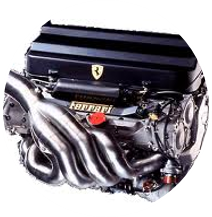
\includegraphics{images/performance.png}
  %\caption{}
	%\label{figure:}
\end{figure}
Améliorer les performances des versions 4.x pour les ramener aux performances de la version 3.1.\\
Les performances critiques étant celles que le client note en premier lieu :
\begin{itemize}
	\item temps d'ouverture d'un document
	\item fonctionnalités de base : création d'un document, sauvegarde, rafra\^{i}chissement
	\item temps de connection au CMS
\end{itemize}


\subsubsection{Intégration continue}
\begin{figure}[H]
  \centering
      
\includegraphics{images/ci.png}
  %\caption{}
	%\label{figure:}
\end{figure}
L'intégration continue doit être assurée de manière à pouvoir détecter le plus tôt possible les régressions (par exemple en compilant ou à chaque livraison de code) et pour pouvoir limiter le risque qu'une compilations casse et de limiter les risques de régressions fonctionnelles en lançant les tests appropriés.\\


\subsubsection{Automatisation}
\begin{figure}[H]
  \centering
      
\includegraphics{images/automation.png}
  %\caption{}
	%\label{figure:}
\end{figure}
Contrôler la qualité de l'héritage inter-versions (compatibilité ascendante) à travers des tests automatiques et assurer la qualité des fonctionnalités en cours de développement.\\
\begin{itemize}
	\item import d'un document créé sur une version 3.x vers une version 4.x
	\item préserver les fonctionnalités et les performances
\end{itemize}

\subsubsection{Optimisation de l'exécution des tests}
\begin{figure}[H]
  \centering
      
\includegraphics{images/produitisation.png}
  %\caption{}
	%\label{figure:}
\end{figure}
Optimiser la couverture de test basée sur les livraisons. \\
Ne pas exécuter les tests qui ne sont pas nécessaires et exécuter ceux qui le sont.

\subsubsection{1 bug = 1 test}
\begin{figure}[H]
  \centering
      
\includegraphics{images/bugtest.png}
  %\caption{}
	%\label{figure:}
\end{figure}
Améliorer la couverture de test de régression en intégrant les anomalies trouvés par les clients dans les fonctionnalités principales. Autrement dit, dès qu'un bug est trouvé un test sera implémenté pour reproduire le problème de manière automatique pour assurer la non-régression. Ce principe permet, comme son nom l'indique, que chacun des bugs corrig\'{e}s par un d\'{e}veloppeur soit test\'{e} syst\'{e}matiquement et automatiquement par un ST\index{Software Tester}.

\subsubsection{Augmenter la couverture de test}
\begin{figure}[H]
  \centering
      
\includegraphics{images/testcoverage.png}
  %\caption{}
	%\label{figure:}
\end{figure}
Trouver les problèmes nouveaux et pas encore découverts en complétant les tests existants, en se concentrant sur les zones à risque.

\subsubsection{ADEPT}
\begin{figure}[H]
  \centering
      
\includegraphics{images/adept.png}
  %\caption{}
	%\label{figure:}
\end{figure}
Réduire le temps de configuration de l'environnement de développement en fournissant des environnement prêts à l'emploi (comprenant IDE, outils de test, codes source, ...) pour toutes les branches BI 4.x.

\subsubsection{Outil de validation des rapports}
\begin{figure}[H]
  \centering
      
\includegraphics{images/validationtool.png}
  %\caption{}
	%\label{figure:}
\end{figure}
Faciliter la migration des clients de la BI4.1 à la BI4.2 en accélérant l'inspection des rapports Web Intelligence après une mise à jour.



